\documentclass[a4paper]{scrartcl}
\usepackage{amsmath,amssymb,graphicx,amsthm, amssymb, amsfonts}
\usepackage{multicol}

\usepackage[utf8]{inputenc}
\usepackage[english]{babel}

\usepackage[x11names,svgnames,dvipsnames]{xcolor}

\usepackage{float}
\usepackage{multicol}  
%\usepackage[rflt]{floatflt}  
\usepackage{graphics}
\usepackage{epsfig} 
%\usepackage{qtree} 
\usepackage{textcomp}
\usepackage{url}

% PDF Import support
\usepackage{pdfpages}
% Support for PDF scaling
\usepackage{graphicx}
% Algorithmen
\usepackage{algorithmic}
\usepackage{algorithm}
\usepackage{listings} 
% \lstset{numbers=left, numberstyle=\tiny, numbersep=5pt} 
\lstset{
	basicstyle=\ttfamily\scriptsize\mdseries,
	keywordstyle=\bfseries\color{blue},
	identifierstyle=,
% 	stringstyle=\itshape\color{red},
	numbers=left,
	numberstyle=\tiny,
	stepnumber=10,
	breaklines=true,
	frame=none,
	showstringspaces=false,
	tabsize=4,
% 	backgroundcolor=\color{gray},
% 	morecomment=[s][\color{green}]{/+}{+/},
	commentstyle=\color{gray},	
	captionpos=b,
	float=htbp,
}
\newcommand{\norm}[1]		{\left|\left| #1 \right|\right|}
\newcommand{\mbf}[1]		{\mathbf{#1}}

\newcommand{\K}     {\mathbb{K}}

%%% Nice Blockquote from 
%% http://tex.stackexchange.com/questions/16964/block-quote-with-big-quotation-marks
% \usepackage[svgnames]{xcolor}

  \usepackage[utf8]{inputenc}
  \usepackage[T1]{fontenc}
  \usepackage{libertine} % or any other font package (or none)
  \newcommand*\quotefont{\fontfamily{fxl}} % selects Libertine for quote font
\usepackage{tikz}
\usepackage{framed}
% Make commands for the quotes
\newcommand*{\openquote}{\tikz[remember picture,overlay,xshift=-15pt,yshift=-12pt]
     \node (OQ) {\quotefont\fontsize{60}{60}\selectfont``};\kern0pt}
\newcommand*{\closequote}{\tikz[remember picture,overlay,xshift=15pt,yshift=10pt]
     \node (CQ) {\quotefont\fontsize{60}{60}\selectfont''};}
% select a colour for the shading
\definecolor{shadecolor}{named}{LightGoldenrodYellow}
% wrap everything in its own environment
\newenvironment{shadequote}%
{\begin{snugshade}\begin{quote}\openquote}
{\hfill\closequote\end{quote}\end{snugshade}}
%% End Blockquote

\newcommand\novspace{\@minipagetrue}
\newtheorem*{definition}{Definition}
\newtheorem*{theorem}{Theorem}

\let\oldemph\emph
\renewcommand{\emph}[1]{{\color{DeepSkyBlue4}{\oldemph{#1}}}}

% redefine greek letters
\renewcommand{\phi}{\varphi}
\renewcommand{\epsilon}{\varepsilon}

% shortcuts in math mode
\newcommand{\bs}{\boldsymbol}
\newcommand{\mc}{\mathcal}
\newcommand{\ds}{\displaystyle}
%\DeclarePairedDelimiter\absimpl{\lvert}{\rvert}
%\DeclarePairedDelimiter\normimpl{\lVert}{\rVert}
\newcommand{\abs}[1]{\absimpl*{#1}}
\newcommand{\norm}[1]{\normimpl*{#1}}
\newcommand{\argmax}{\operatorname*{arg\,max}}
\newcommand{\argmin}{\operatorname*{arg\,min}}

% number sets
\newcommand{\R}{\mathbb{R}}
\newcommand{\Z}{\mathbb{Z}}
\newcommand{\N}{\mathbb{N}}
\newcommand{\Q}{\mathbb{Q}}
\newcommand{\C}{\mathbb{C}}
\newcommand{\F}{\mathbb{F}}
\newcommand{\LL}{\mathcal{L}}
\newcommand{\powerset}{\mathcal P}
\newcommand{\normal}{\mathcal N}

\newcommand{\sectionline}{\noindent\makebox[\linewidth]{\rule{\columnwidth}{0.1pt}}}
\newcommand{\msection}[1]{\vspace{-1mm}\sectionline\vspace{-1mm}\section{#1}\vspace{-1mm}}
% probabilities
\newcommand{\Prob}[1]{\operatorname{Pr}\left[#1\right]}
\newcommand{\Ex}[1]{\mathbb{E}\left[#1\right]}

% misc
\newcommand{\bigO}[1]{\mc O\left(#1\right)} % big-o notation

\newcommand{\nop}[1]{} % temporarily remove from output

% remove the paragraph indentation
 \setlength{\parindent}{0in}

\author{Pascal Spörri\\pascal@spoerri.io}
\title{Physically Based Simulation\\Summary HS 2012}
%\thanks{Licence: Creative Commons Attribution-Share Alike 3.0 Unported (\url{http://creativecommons.org/licenses/by-sa/3.0/})}}
\date{\today}
\usepackage[colorlinks=false,pdfborder = {0 0 0 0}]{hyperref}


\begin{document}
\maketitle
\newpage

\part{Mass-Spring Systems}
\begin{multicols}{2}
Steps towards a simulation of a Mass-Spring system:
\begin{itemize}
\item \emph{Spatial discretization}: Sample object with mass points
\item \emph{Forces}: Define internal (springs!) and external forces
\item \emph{Dynamics}: Set up equations of motion
\item \emph{Temporal discretization}: Solve equations of motion
\end{itemize}

\section{Spatial Discretization}
    Sample object with mass points:
    \begin{align*}
    	\text{Total mass of object: }& M,\\
    	\text{Number of mass points: }& n,\\
    	\text{Mass of each point: }& m = {M \over n},
    \end{align*}
    with each point holding the properties:
    \begin{align*}
    	\text{Mass: }&m_i\\
    	\text{Position: }& x_i(t)\\
    	\text{Velocity: }& v_i(t) 
    \end{align*}

\section{Forces}
 What are the forces that act on particle $i$?
	\begin{description}
		\item[External Forces] Gravity: $F_i$
		\item[Internal Forces] $\textbf{}$
			\begin{itemize}
				\item Elastic spring forces
				\item Viscous damping forces
			\end{itemize}
		\item[Total force] $F_i = F_i^{int} + F_i^{ext}$
	\end{description}

\subsection{Internal Forces}
\subsubsection{Elastic Springs}
\begin{definition}[Elasticity]
	Ability of a spring to return to its initial length when the deforming force is removed. 
\end{definition}

\begin{align*}
	F & =-k(l-L) & \text{Hooke's Law } (1D)\\
	F_i &= -k(||\vec x_i - \vec x_j || - L) {\vec x_i - \vec x_j \over ||\vec x_i - \vec x_j || } & (3D)\\
	L: &\quad \text{ Initial spring length}\\
	l: &\quad \text{ Current spring length}\\
	k: &\quad \text{ Spring stiffness}
\end{align*}
For purely elastic springs \emph{the force depends only on the position} and \emph{no energy is lost during the deformation}.
\begin{align*}
	W &=\int_L^l k(x-L) dx &\text{Work done by forces}\\
	E &= W= {1 \over 2} k(l-L)^2 &\text{Elastic spring energy}\\
	\vec F_i &= -{\del E \over \delta \vec x_i} &\text{Force}
\end{align*}

\paragraph{Forces at Mass Point} internal forces $F_0^{int}$:
\begin{align*}
	\vec F_0^{int} &= -\sum_{i|i\in \{1,2,3\}} k_i (l_i-L_i) {\vec x_i - \vec x_0 \over l_i}
\end{align*}
\begin{figure}[H]
	\centering
	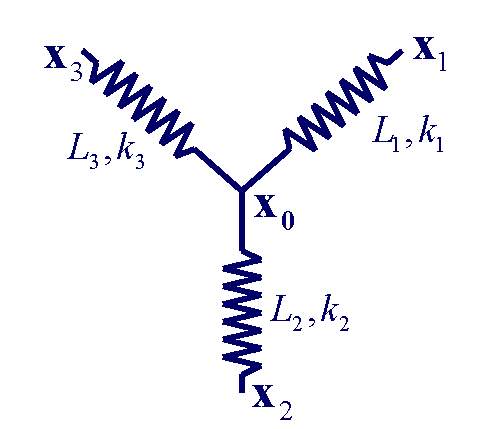
\includegraphics[width=0.4\textwidth]{img/01_forces_at_mass_point.pdf}
	\caption{Example}
\end{figure}

\subsection{Dissipative Forces}
Real-world mechanical systems dissipate energy over time: \emph{Internal friction $\implies$  Thermal energy} (irreversible process). Controllable dissipation is useful for physics simulations. 
\paragraph{Dissipation for mass-spring systems} $\gamma$ is the damping coefficient
\begin{align*}
\vec F^{pd} (t) &= -\gamma\cdot \vec v(t) &\text{Point damping}
\end{align*}
Point damping is simple and efficient, but it \emph{damps \textbf{all} motion} (i.e. including translations and rotations).

\subsection{External Forces}
External forces are forces like
\begin{itemize}
	\item Gravity
	\item Contact forces
	\item All forces that are not cause by springs
\end{itemize}

\section{Dynamics}
In the dynamics step the equations of motion are setup. The force is known for every particle.
    \paragraph{Kinematic relations}
		\begin{align*}
			\textbf{Velocity: }\vec v_i(t) &= {d \vec x_i (t) \over dt}\\
			\textbf{Acceleration: }\vec a_i(t) &= {d\vec v_i(t) \over dt} = {d^2 \vec x_i(t) \over dt^2}
		\end{align*}

With \textbf{Newton's $2^\text{nd}$ Law} 
\begin{align*}
\vec F_i &=m_i \cdot \vec a_i
\end{align*}
we can describe the equations of motion using Newton's second law:
\begin{align*}
	\vec F_i &= m_i {d^2 \vec x_i (t) \over d t^2} = \vec F_i^{int}(t) + \vec F_i^{ext}(t)\\
	&\text{which can be abstracted as}\\
	\vec F  &= M {d^2 \vec x (t) \over d t^2} = \vec F^{int}(t) + \vec F^{ext}(t) & M \in \R^{3n\times 3n}\\
	&\text{adding damping}\\
&	M {d^2 \vec x (t) \over d t^2} + D {d\vec x(t) \over dt}= \vec F^{int}(t) + \vec F^{ext}(t)
\end{align*}

\section{Temporal discretization}
A \emph{differential equation} describes an unknown function through its derivatives. An ordinary differential equation (ODE) contains only derivatives with respect to a single variable.

\begin{tabular}{c|c}
	\textbf{Example}&\textbf{Abstract form}\\ \hline
	$x''(t) = {\vec F(t) - \gamma \vec x'(t) \over m_i}$&
	$y''(t) = f(t, y, y')$
\end{tabular}
The order of the ODE is expressed as function of the highest derivative:
\begin{align*}
	y^{(n)} = f(x, y, y',y'',\ldots,y^{(n-1)}).
\end{align*}

Solving an ODE: Given $f$, determine $y$. Example:
\[
	y'(t) = f(t,y) = y(t) \quad \Longrightarrow\quad y(t) = Ce^t
\]
The integration constant $C$ is unknown and i determined by the initial value:
\begin{align*}
	y(0) =2 \qquad \Longrightarrow \qquad C = 2
\end{align*}
\emph{ODE + initial value = initial value problem (IVP)}

\begin{theorem}{Picard–Lindelöf}
An IVP has a unique solution if $f$ is Lipschitz continuous.
\end{theorem}
\subsection{Application to Mass-Spring systems}
We have an initial position $\vec x_i(t_0)$, an initial velocity $\vec v_i (t_0)$ and a governing ODE:
\begin{align*}
	{d^2 \vec x_i (t) \over dt^2} = {\vec F_i(t) - \gamma \vec v_i(t) \over m_i}.
\end{align*}
We want the position $\vec x_i$ over time. 

The first step to rewrite the problem since it's easier to deal with as a first oder ODE. We therefore reduce the $2^{nd}$ order ODE to two coupled $1^{st}$ order ODEs.
\begin{align*}
	&m_i {d^2 \vec x_i(t) \over dt^2} + \gamma {d \vec x_i (t) \over dt} = \vec F_i (t) \\
	&\begin{cases}
		{d \vec x_i(t) \over dt} = \vec v_i (t) & \text{velocity} \\
		{d \vec v_i(t) \over dt} = {\vec F_i (t) - \gamma \vec v_i (t) \over m_i} & \text{acceleration}
	\end{cases}
\end{align*}

Write as one system of $1^{st}$ order ODEs:
\begin{align*}
	\vec y_i (t) &= \begin{pmatrix}
 						\vec x_i(t)\\
 						\vec v_i(t)
 					\end{pmatrix}\\
	\vec y_i' (t) &=  \begin{pmatrix}
  						\vec v_i(t)\\
  						{\vec F_i (t) - \gamma \vec v_i (t) \over m_i}
  					   \end{pmatrix}
\end{align*}

\subsection{Numerical Solution}
Compute approximations $y_i$ to true solution for \emph{discrete} time instants $t_i$. Compute solution at $t_{i+1}$ based on previous solutions at $t_{i-1}$, $t_{i-2}$.
\begin{figure}[H]
	\centering
	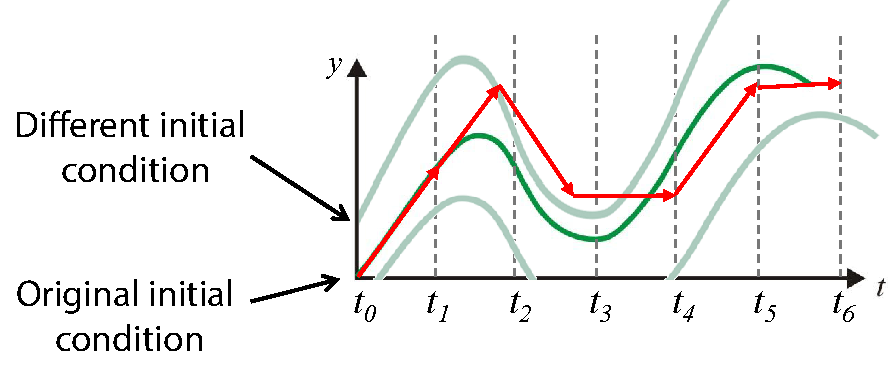
\includegraphics[width=0.45\textwidth]{img/01_initial_conditions}
	\caption{Solutions based on different initial conditions}
\end{figure}

\section{Integration schemes} $\textbf{}$
\begin{description}
	\item[Explicit Methods] $\textbf{}$
		\begin{itemize}
			\item Explicit Euler
			\item Heun, Midpoint
			\item Runge-Kutta methods
		\end{itemize}
		Tend to explode with \emph{stiff problems}:
		\begin{itemize}
			\item Explicit methods require very small time steps for stable integration
			\item Are inefficient since step size is determined by stability not accuracy requirements. 
		\end{itemize}
		Use implicit methods for stiff problems.
	\item[Implicit Methods] $\textbf{}$
		\begin{itemize}
			\item Backward Euler
			\item Implicit Euler
			\item BDF methods
		\end{itemize}
	\item[Methods for higher order ODEs] $\textbf{}$
		\begin{itemize}
			\item Verlet
			\item Leapfrog
			\item Newmark methods
		\end{itemize}
\end{description}

\subsection{Computing Approximations} An approximation of a function $y(t)$ can be computed by computing the taylor expansion:
\begin{align*}
	y(t+h) &= y(t) + {y'(t) \over 1!}h + {y''(t) \over 2!}h^2 + \ldots,
\end{align*}
which allows us to compute a first order approximation:
\begin{align*}
	y(t+h) &= y(t) + hy'(t).
\end{align*}
Which leaves us with \emph{Euler' Method}.

\subsubsection{Accuracy criteria} to evaluate an integration scheme:
\begin{description}
	\item[Convergence] Do approximations converge to true solution, i.e. 
		\[
			h\mapsto 0 \implies y_i \mapsto y_i(t)
		\]
	\item[Accuracy] how fast does the error decrease as $h\mapsto 0$\\
		Local error is $\bigO{h^{p+1}}$ $\implies$ Method is accurate of order $\mathbf p$.
	\item[Stability] Is the solution always bounded, i.e. $|y_n| < \infty$
	\item[Efficiency] Is a given method a good choice for a given problem?
\end{description}

\subsection{Integration Schemes}

\subsubsection{Euler's Method} Start at the initial condition and take a step into the direction of the tangent.
\begin{align*}
	y_{n+1} &= y_n + hf(t_n, y_n).
\end{align*}

\begin{figure}[H]
	\centering
	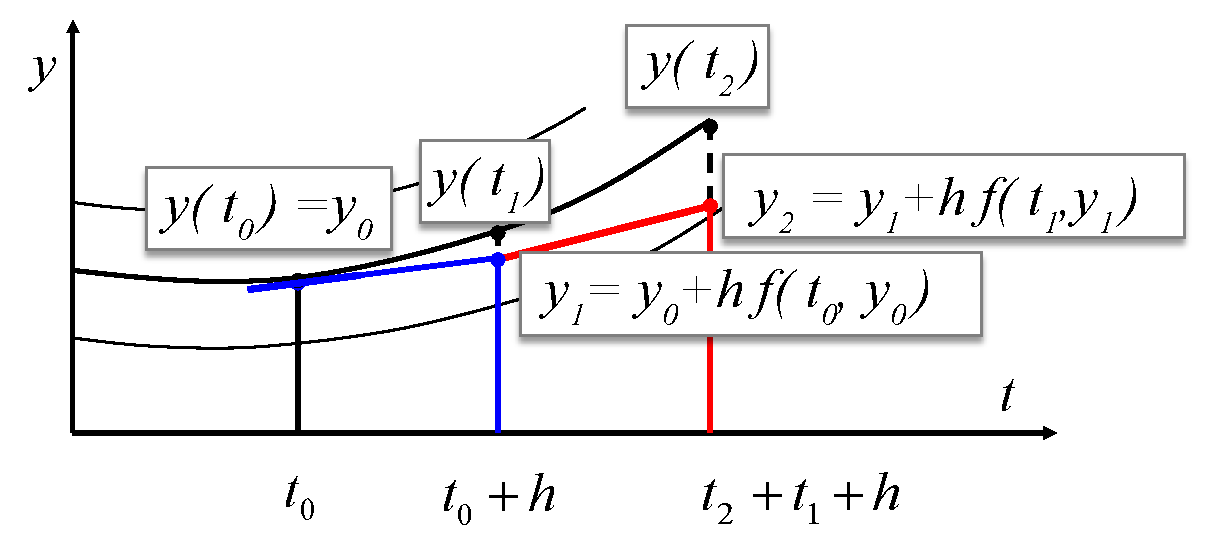
\includegraphics[width=0.45\textwidth]{img/01_euler}
	\caption{Visualization of the Euler Method}
\end{figure}

Explicit Euler has an accuracy of order $1$: $\bigO{h^2}$ error per stop.


\subsubsection{Heun's Method}
Heun's method is a two step method and provides a $\mathbf{2^{nd}}$ \textbf{order accuracy}. Idea:
\[
	y(t+h) \approx y(t) + {h \over 2} [y'(t) + y'(t+h)],
\]
$y'(t+h)$ is unknown. Use an Euler step to compute it. 
\begin{align*}
	\tilde y_{n+1} &= y_n + h\cdot f(t_n, y_n) \\
	y_{n+1} &= y_n + {h \over 2} \left[ f(t_n, y_n) + f(t_{n+1}, \tilde y_{n+1}) \right]
\end{align*}

\begin{figure}[H]
	\centering
	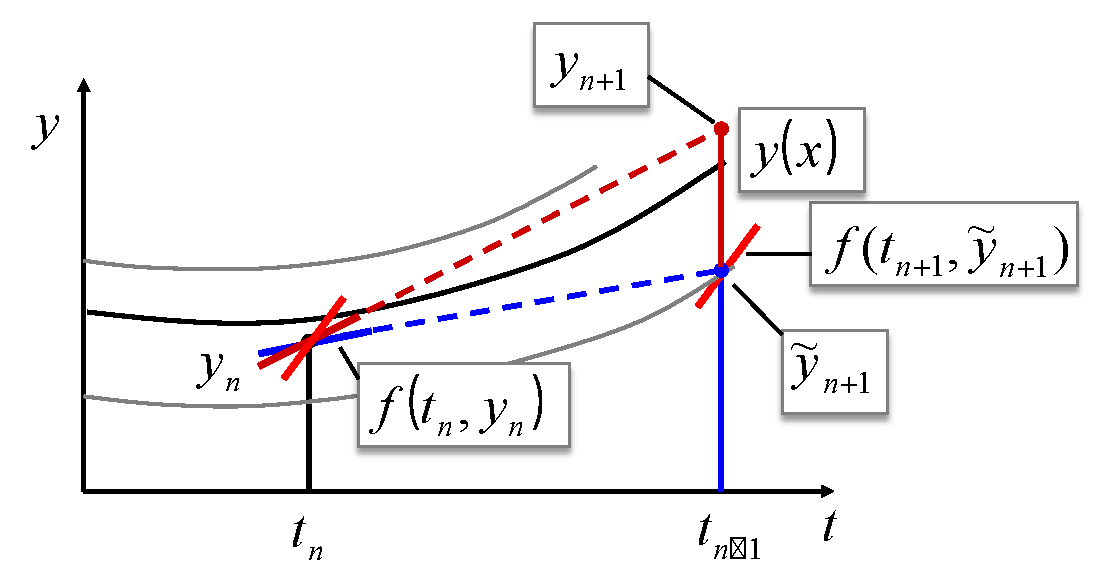
\includegraphics[width=0.45\textwidth]{img/01_heun}
	\caption{Heun's Method graphically}
\end{figure}

\subsubsection{Explicit Midpoint Method}
Heun's method uses $f(t)$ and $f(t+h)$ to achieve $2^{nd}$ order accuracy. Use $f\left(t+{h\over 2} \right)$ instead. This also gives us $2^{nd}$ order accuracy.

\begin{align*}
	\tilde y_{n+1} &= y_n + {h \over 2}\cdot f(t_n, y_n) \\
	y_{n+1} &= y_n + h \left[ f(t_n, y_n) + f(t_{n+1}, \tilde y_{n+1}) \right]
\end{align*}
This solution provides us also with provides a $\mathbf{2^{nd}}$ \textbf{order accuracy}.

\subsubsection{$\mathbf{4^{th}}$-Order Runge-Kutta}
\emph{RK4} is one of the most widely used integrators. Four slope evaluations gives us $\mathbf{4^{th}}$ \textbf{order accuracy}
\begin{align*}
	k_1 &= f\left(t_n, y_n\right)\\
	k_2 &= f\left(t_n+{1\over 2}h, y_n+{1\over 2}k_1\right)\\
	k_3 &= f\left(t_n+{1\over 2}h, y_n+{1\over 2}k_2\right)\\
	k_4 &= f\left(t_n+h, y_n + h k_3\right)
\end{align*}
$y_{n+1}$ is computed using a weighted average slope:
\begin{align*}
	y_{n+1} &= y_n + {1 \over 6}h (k_1 + 2k_2 + 2k_3+k_4)
\end{align*}
\begin{figure}[H]
	\centering
	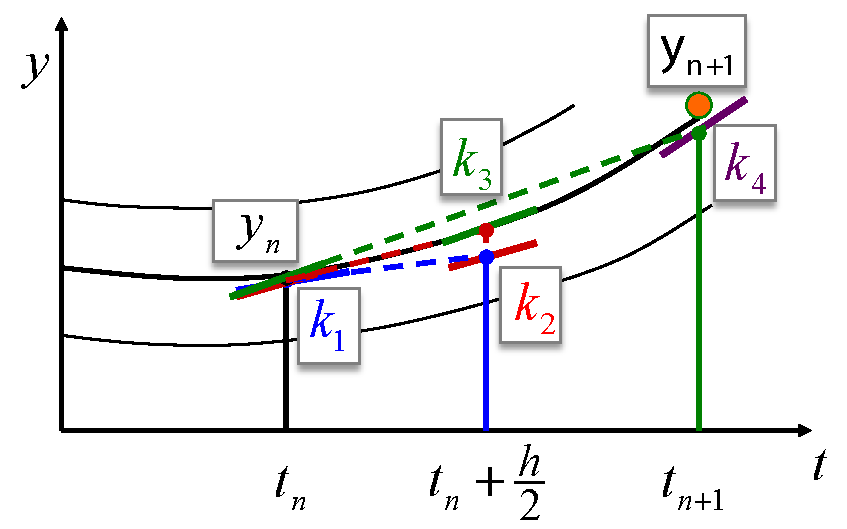
\includegraphics[width=0.45\textwidth]{img/01_rk4}
	\caption{RK4 graphically}
\end{figure}

\subsubsection{Implicit Euler Method}

\begin{align*}
	y_{n+1} &= y_n + hf(t_{n+1}, y_{n+1})
\end{align*}
Implicit methods have to be solved iteratively. Example with Newton's method:
\begin{enumerate}
	\item \textbf{Rewrite equation}:
	
		\begin{align*}
			0 = y_{n+1} - y_n - hf(t_{n+1}, y_{n+1}) = g(y_{n+1})
		\end{align*}
	\item \textbf{Make initial guess}:
		\begin{align*}
			\tilde y_{n+1} = y_n
		\end{align*}
	\item \textbf{Taylor expansion}:
	
		\begin{align*}
			g(\tilde y_{n+1}+\Delta y) = g(\tilde y_{n+1}) + g'(\tilde y_{n+1}) + \bigO{\Delta y^2} = 0
		\end{align*}
		
	\item \textbf{Linearize}
	
		\begin{align*}
			g'(\tilde y_{n+1} \cdot \Delta y = -g(\tilde y_{n+1})
		\end{align*}
\end{enumerate}
In order to solve the equation one has to iterate over
\begin{align*}
	\Delta y &=	-{g(\tilde y_{n+1}) \over g'(\tilde y_{n+1}) } & \text{Solve},\\
	\tilde y_{n+1} &= \tilde y_{n+1} + \Delta y &\text{Update},\\
	r &= g(\tilde y_{n+1}) &\text{Error},
\end{align*}
until the \emph{Error} is small enough.\\

Newton's method is powerful, but it has to be used with care:
\begin{itemize}
	\item Requires the computation of the solution of a linear system in each iteration.
	\item A robust implementation needs advanced strategies.
\end{itemize}

\subsubsection{Semi-Implicit Euler Method}
The \emph{semi-implicit} Euler method can be applied to a pair of \emph{differential equations} of the form:
\begin{align*}
	{dx \over dt} &= f(t,v)\\
	{dv \over dt} &= g(t,x)
\end{align*}
The discrete solution can be computed by iterating over:
\begin{align*}
	v_{n+1} &= v_n + g(t_n, x_n)\Delta t\\
	x_{n+1} &= x_n + f(t_n, v_{n+1})\Delta t
\end{align*}

\subsection{Higher-Order Numerical Integration}
Let 
\begin{align*}
	M\ddot x = F^{int} + F^{ext}
\end{align*}
\subsubsection{Verlet Integration}
Combine forward and backward expansions of $x(t)$. Which results in a $\mathbf{2^{nd}}$ \textbf{order method}.

\begin{align*}
	&\  \ \begin{cases}
	x(t+h) &=  x(t) + hx'(t) + {h^2\over 2}a(t) + {h^6 \over 6} x'''\\ 
	x(t+h) &=  x(t) - hx'(t) + {h^2\over 2}a(t) / {h^6 \over 6} x'''
	\end{cases}\\
	&x(t+h) = 2 x(t) - x(t-h) + h^2a(t) 
\end{align*}

\begin{itemize}
	\item The two-step method makes it problematic for discontinuities.
	\item \emph{Velocities} have to be \emph{approximated a posteriori}.
\end{itemize}


\subsubsection{Leapfrog}
Compute velocities on a \emph{staggered grid}. $\mathbf{2^{nd}}$ \textbf{order method}.
\begin{align*}
	v\left(t+{h \over 2}\right) &= v \left(t - {h\over 2}\right) + h\cdot a(t)\\
	x(t+h) &= x(t) + h\cdot v\left( t + {h\over 2} \right)
\end{align*}
This method is only applicable if $a(t)$ does not depend on velocity: $\implies$ no damping!

\subsubsection{Symplectic Euler}
$\mathbf{2^{nd}}$ \textbf{order accurate}
\begin{align*}
	v(t+h) &= v(t) + h\cdot a(t)\\
	x(t+h) &= x(t) + h\cdot v(t+h)
\end{align*}

Has a good stability for oscillatory motion and good conservation properties:
\begin{itemize}
	\item Exactly conserves momentum
	\item Nearly conserves energy over long run times.
\end{itemize}

\section{A Basic Mass-Spring System}
\subsection{Setting up Springs}
Is the model provided as tetrahedral mesh?
\begin{description}
	\item[Yes:] Model edges as springs
	\item[No:] Find \emph{stable} topology:
		\begin{itemize}
			\item No control over material properties
			\item No explicit volume preservation.
		\end{itemize}
\end{description}

\paragraph{Springs for Cloth} Types of require springs:
\begin{figure}[H]
	\centering
	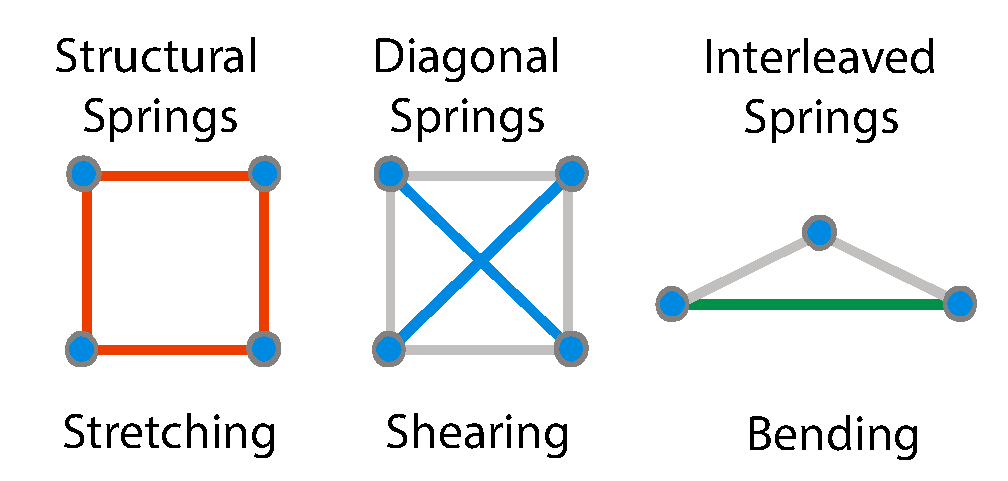
\includegraphics[width=0.45\textwidth]{img/02_springs_cloth}
	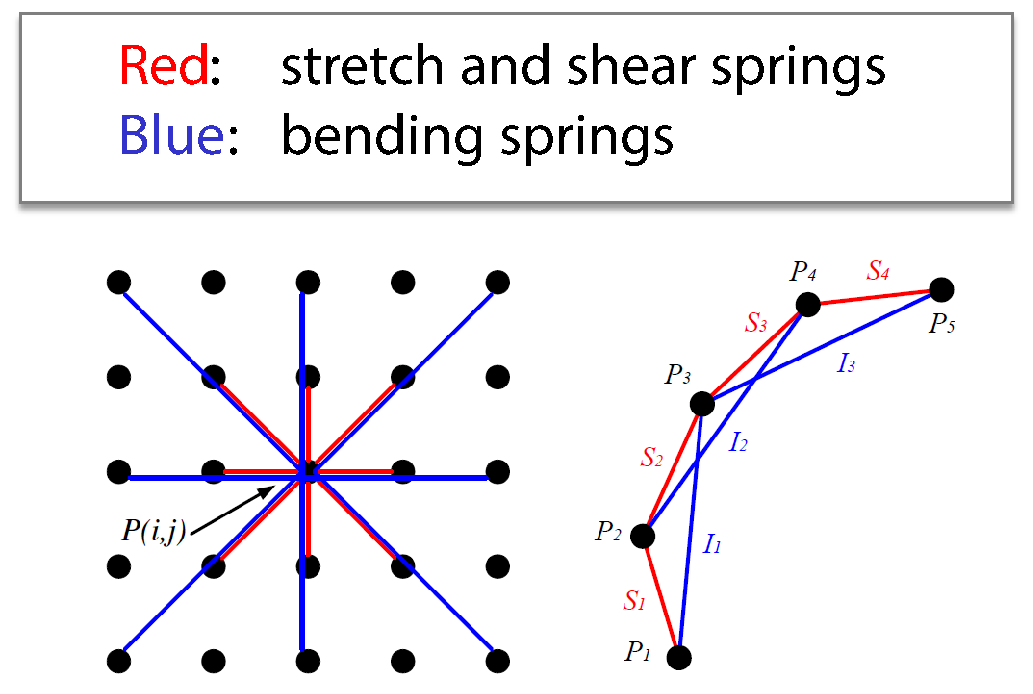
\includegraphics[width=0.45\textwidth]{img/02_springs_cloth_2}
\end{figure}
Springs couple different deformation modes:
\begin{itemize}
	\item Bending and shear springs respond to stretch,
	\item Which lead to uncontrollable transverse contraction.
\end{itemize}
\begin{figure}[H]
	\centering
	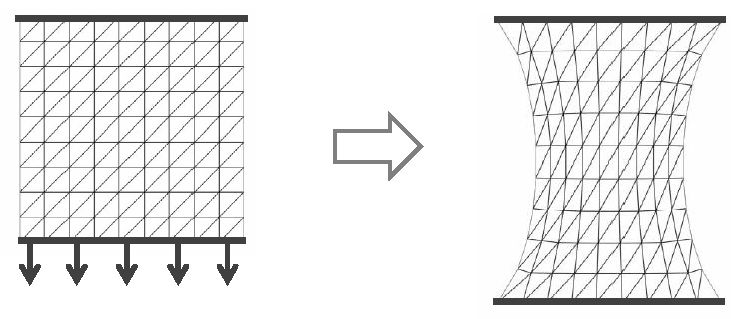
\includegraphics[width=0.45\textwidth]{img/02_contraction}
	\caption{Transverse Contraction due to bending and shear springs}
\end{figure}

The material behaviour depends strongly on topology.
\begin{figure}[H]
	\centering
	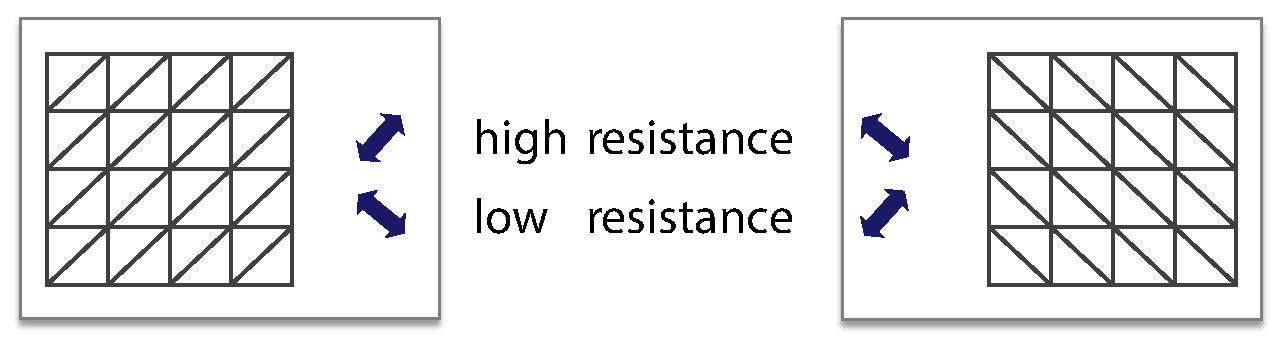
\includegraphics[width=0.45\textwidth]{img/02_material_behaviour}
	\caption{Material behaviour}
\end{figure}

\paragraph{Limitations}
\begin{itemize}
	\item Strong dependence on discretization (topology)
	\item Limited control over material behaviour
	\item No (explicit) volum preservation (for solids)
\end{itemize}

\paragraph{Verdict} Mass-Spring Systems are simple and efficient, but not very accurate.
\paragraph{Alternatives}
\begin{itemize}
	\item Constraints
	\item Continuum-mechanics with Finite Elements
\end{itemize}



\end{multicols}

\newpage
\part{Constraints}
\begin{multicols}{2}
So far, the motion of particle was defined by forces:
\begin{itemize}
	\item Elastic springs,
	\item Damping,
	\item Gravity
\end{itemize}
motion is unrestricted using these techniques. Sometimes we want to restrict motion:
\begin{itemize}
	\item Bead a wire (constant length),
	\item Incompressible deformations (constant volume).
\end{itemize}
 \emph{Constraints} can be use to strictly \emph{enforce conditions} (unlike elastic forces) or to \emph{derive general forces} (unlike springs).

\begin{definition}{Constraint}
	A constraint $C(x_1, x_2, \ldots, x_n)$ is 
	\begin{itemize}
		\item A scalar-valued function of one or several arguments
		\item An implicit expression for a relation that must hold between its arguments.
	\end{itemize}

	\textbf{Convention}: A constraint is satisfied if $\mathbf{C=0}$.
\end{definition}
Examples of $n$-ary constraints:
\begin{itemize}
	\item Constant position $C_1(x_1)$
	\item Constant length $C_2(x_1, x_2)$
	\item Constant area $C_3(x_1, x_2, x_3)$
	\item Constant volume $C_4(x_1, x_2, x_3, x_4)$
\end{itemize}
\begin{figure}[H]
	\centering
	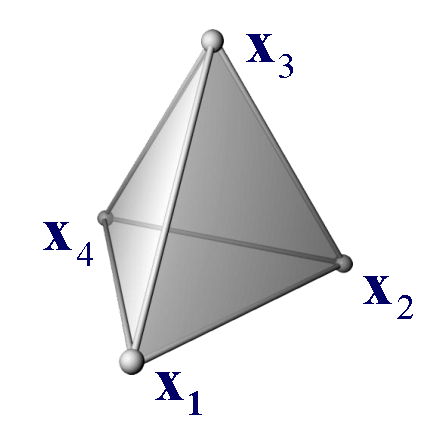
\includegraphics[width=0.25\textwidth]{img/02_tetra}
\end{figure}

\section{Soft constraints and the Penalty Method}
How can we enforce constraints? \\

Define potential energy for constraint:
\begin{align*}
	E_c(x_1, x_2, \ldots, x_n) = {1 \over 2} kC(x_1, x_2, \ldots, x_n)^2,
\end{align*}
where $k$ is a \emph{stiffness} coefficient.
\begin{align*}
	E_c &= 0 &\text{constraint is met},\\
	E_c &> 0 &\text{otherwise}.
\end{align*}
The \emph{constraint force} is a \emph{negative gradient} of potential energy:
\begin{align*}
	F_j = - {\delta E_c \over \delta x_j} = - kC(x_1, \ldots x_n){\delta C(x_1,\ldots, x_n) \over \delta x_j}
\end{align*}
The \emph{penalty force} pulls the system towards $\mathbf{C=0}$.

\paragraph{Distance Preservation} Preserve distance between two points:
\begin{align*}
	C(x_0, x_1) &= \norm{x_1-x_0}-L\\
	F_1^C(x_0, x_1) &= -kC(x_0, x_1){\delta C(x_0, x_1) \over \delta x_1}\\
		&= \underbrace{-k(\norm{x_1-x_0}-L){x_1-x_0 \over \norm{x_1-x_0}}}_\textbf{Spring Force}
\end{align*}

\paragraph{Simulation with Penalty Forces} Simulate $x_0$ and $x_1$ using Newton's law. Enforce distance constraint with penalty forces:
\begin{align*}
 F_i^C(x_0, x_1) &= -kC(x_0, x_1){\delta C(x_0, x_1) \over \delta x_i}
\end{align*}
Step forward in time (explicit Euler):
\begin{align*}
	v_{n+1} = v_n + h {1 \over M}\left( F^C (x) + F^{ext} \right).
\end{align*}
\end{multicols}

\subsubsection{Recipes for constraint forces}
\begin{description}
	\item[Area of a triangle] $(x_0, x_1, x_2)$:
		\begin{align*}
			C(x_0, x_1, x_2) = {1\over 2} \norm{(x_1-x_0) \times (x_2-x_0)}-A
		\end{align*}
	\item[Volume $\mathbf V$ of a tetrahedron] $(x_0, x_1, x_2, x_3)$:
		\begin{align*}
			C(x_0, x_1, x_2, x_3) = {1\over 6} (x_1-x_0) \cdot \left[ (x_2-x_0) \times (x_3-x_0) \right]-V
		\end{align*}
\end{description}

\subsection{Summary Soft Constraints}
Constraint forces are:
\begin{itemize}
	\item A powerful mechanism to enforce various conditions,
	\item Generic: Express condition, forces from a standard scheme,
	\item $n$-ary forces as opposed to binary strings.
\end{itemize}

\emph{However}, constraints can be:
\begin{itemize}
	\item Computationally expensive (especially with implicit integration),
	\item Redundant or conflicting,
	\item Penalty forces \emph{model \textbf{soft} constraints} and are \emph{not sufficient} for strict enforcement (\emph{\textbf{hard} constraints}).
\end{itemize}

\begin{multicols}{2}
\section{Hard Constraints}
How can we model a hard constraint? Consider a 2D particle constrained to move on a unit circle.
\begin{figure}[H]
\centering
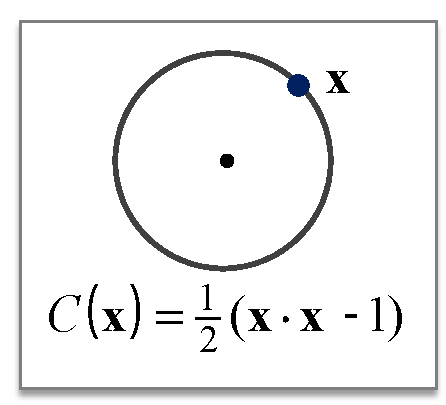
\includegraphics[width=0.40\textwidth]{img/02_hard_constraints_circle}
\end{figure}
First we define \emph{legal} kinematics:
\begin{align*}
	\textbf{Position: }&C(x) = 0\\
	\textbf{Velocity: }&\dot C(x) = 0\\
	\textbf{Acceleration: }&\ddot C(x) = 0
\end{align*}
\textbf{Idea:} Start with a legal position and velocity and ensure that acceleration remains legal (constraint forces).
\begin{align*}
	&\begin{cases}
	\underbrace{\ddot C(x) = \ddot x \cdot x + \dot x \cdot \dot x = 0}_\text{Legal acceleration}\\
	\underbrace{ \ddot x = {F + F^C \over m} }_\text{Newton's Law}
	\end{cases}\\
	 &\text{combine:}\\
	&F^C \cdot x = -F\cdot x - m\dot x \cdot \dot x
\end{align*}
Require constraint force to act only in gradient direction:
\begin{align*}
	F^C = \lambda {\delta C \over \delta x} = \lambda x.
\end{align*}
Insert into combined formula:
\begin{align*}
	\lambda = - {F\cdot x + m \dot x \cdot \dot x \over x \cdot x},
\end{align*}
which gives us an \emph{hard constraint force}.

\paragraph{Simulation with Hard Constraints} Use hard constraints with an explicit function (since implicit integration is (much) more complicated):
\begin{enumerate}
	\item Solve (LES) for constraint force magnitudes $\lambda_n$.
	\item Compute constraint forces:
		\begin{align*}
			F_n^C &= {\delta C(x_n)^t \over \delta x}\lambda_n
		\end{align*}
	\item Step forward in time 
		\begin{align*}
			v_{n+1} = v_n + {h\over M} \left(F_n^C + F^{ext}\right)
		\end{align*}
\end{enumerate}

\subsection{Summary Hard Constraints}
Hard constraint forces
\begin{itemize}
	\item add just enough force to maintain constraint (exactly),
	\item require no high stiffness (numerically pleasing).
\end{itemize}
However
\begin{itemize}
	\item \emph{Constraints drift} (error in ODE solve), needs correction
	\item General formulation is more involved (many constraints)
	\item Requires the solution of systems of equations
\end{itemize}





\end{multicols}



\end{document}